%%%%%%%%%%%%%%%%%%%%%%%%%%%%%%%%%%%%%%%%%%%%%%%%%%%%%%%%%%
% Template para redação de Teses/Dissertações da ESALQ/USP
% Autor: Antonio Augusto Franco Garcia
%%%%%%%%%%%%%%%%%%%%%%%%%%%%%%%%%%%%%%%%%%%%%%%%%%%%%%%%%%

% Este arquivo concatena todos os arquivos individuais e o template

% ESTE É O ARQUIVO QUE DEVE SER COMPILADO!!!!!

% AS CONFIGURAÇÕES NESTE ARQUIVO NÃO DEVEM SER ALTERADAS
% INADVERTIDAMENTE. MUDE APENAS O QUE FOR EXPLICITAMENTE INDICADO.

% Preâmbulo: definição da classe e inclusão do template
% NÃO MUDE NADA AQUI, NEM O TAMANHO DA FONTE
\documentclass[book,A4paper,10pt,twoside,oldfontcommands]{memoir}
\usepackage{./template/Template_Tese}


% Inclua aqui a lista dos pacotes do LaTeX que você necessita usar.
% Por exemplo, para incluir o pacote amsmath, remova o comentário da
% linha correspondente logo abaixo. Insira os demais pacotes de forma análoga.
% ATENÇÃO: alguns pacotes são incompatíveis entre si, ou se sobrepõem
% as configurações de outros; use com cuidado
% amsmath: \usepackage{amsmath}


%%%%%%%%%%%%%%%%%%%%%%%%%%%%%%%%%%%%%%%%%
% Início do documento - Parte Pré-textual
\begin{document}

% Macro da classe memoir que remove os cabeçalhos (comuns em
% documentos da classe "book")
\pagestyle{fnsizeheadings}

% Inclusão do arquivo com informações necessárias para a parte
% pré-textual.
% %%%% 
% VOCÊ DEVE ABRIR O ARQUIVO TodasInformações.tex E
% ALTERÁ-LO DA FORMA APROPRIADA PARA O SEU TRABALHO. 
% %%%%
% Lembre-se de  conferir o número de páginas quando tiver a versão final a ser
% submetida.
%%%%%%%%%%%%%%%%%%%%%%%%%%%%%%%%%%%%%%%%%%%%%%%%%%%%%%%%%%%%%%
% PREENCHA ABAIXO COM AS INFORMAÇÕES NECESSÁRIAS
%%%%%%%%%%%%%%%%%%%%%%%%%%%%%%%%%%%%%%%%%%%%%%%%%%%%%%%%%%%%%%

%%% Título da tese/dissertação
\newcommand{\TítuloDoTrabalho}{%
  Título do trabalho apenas com a primeira letra em maiúsculo, com
  exceção de nomes próprios e científicos (em itálico), sem ponto
  final 
}

%%% Título da tese/dissertação em inglês
\newcommand{\TítuloEmIngles}{%
  Título do trabalho (em inglês) apenas com a primeira letra
  em maiúsculo, com exceção de nomes próprios e científicos (em
  itálico), sem ponto final 
}

%%% Autor (nome completo por extenso)
% OBS: nome exatamente como cadastrado no Sistema Janus
\newcommand{\Autor}{%
  Nome completo do autor 
}

%%% Qual é seu último nome? (Como você usa nas publicações). Se houver
%%% Júnior, Filho, etc, indique apropriadamente. Ex: Silva Filho.
%%% É possível também usar hífen, como p ex Pizzirani-Kleiner.
%%% O Sobrenome de Fulano de Tal é exemplificado abaixo. 
%%% Note a exclusão do "de"
\newcommand{\Sobrenome}{%
  Tal}

%%% Qual é seu primeiro nome, nome do meio, e demais partes do
%%% sobrenome (não incluídas acima)? A soma deste item e do anterior
%%% devem formar seu nome completo por extenso. Não abrevie.
\newcommand{\Nome}{%
  Fulano de
}

%%% Indique o título da graduação que você possui. Ex: Engenheiro Agrônomo
\newcommand{\TituloDaGraduação}{%
  Título da Graduação (como está no diploma)
}

%%%% Indique o nome do seu Orientador (nome completo por extenso)
\newcommand{\Orientador}{%
  Nome completo do orientador
}

%%% Seu orientador(a) é Prof. Dr. ou Profa. Dra.? Selecione umas das
%%% linhas abaixo. Não remova as barras invertidas, apenas selecione a
%%% linha apropriada, comentando a outra
\newcommand{\DoutorOuDoutora}{%
  Prof.\ Dr.\
  %Profa.\ Dra.\
}

%%%% Que título você pretende obter? Indique abaixo, alterando o texto
% Há várias opções; adapte aquela adequada para o seu caso.
%
% A maioria dos programas da ESALQ e CENA segue o padrão abaixo:
%
% Dissertação apresentada para obtenção do título de Mestre (ou Mestra)
% em Ciências. Área de concentração: Verificar no site da CPG (sem
% ponto final) 
%
% Tese apresentada para obtenção do título de Doutor (ou Doutora) em
% Ciências. Área de concentração: Verificar no site da CPG (sem ponto
% final)
% 
% No caso do PPG em Recursos Florestais, selecione abaixo (indicando
% mestrado ou doutorado apropriadamente).
%
% Dissertação (ou Tese) apresentada para obtenção do título de Mestre
% (ou Mestra) ou Doutor (ou Doutora) em Ciências, Programa: Recursos
% Florestais. Opção em: Silvicultura e Manejo Florestal
%
% Dissertação (ou Tese) apresentada para obtenção do título de Mestre
% (ou Mestra) ou Doutor (ou Doutora) em Ciências, Programa: Recursos
% Florestais. Opção em: Tecnologia de Produtos Florestais
%
% Dissertação (ou Tese) apresentada para obtenção do título de Mestre
% (ou Mestra) ou Doutor (ou Doutora) em Ciências, Programa: Recursos
% Florestais. Opção em: Conservação de Ecossistemas Florestais 
%
% PPG International em Biologia Celular e Molecular Vegetal
% 
% Tese apresentada para obtenção do tĩtulo de Doutor (ou Doutora) em
% Ciências. Programa: Internacional Biologia Celular e Molecular Vegetal
% 
\newcommand{\TítuloObtido}{%
  Tese apresentada para obtenção do título de Doutor (ou Doutora) em
  Ciências. Área de concentração: Verificar no site da CPG (sem ponto
  final)
}


%%%%% Tese revisada
% É possível entregar versão revisada de acordo com a resolução CoPGr
% 6018 de 2011. Caso você esteja fazendo isso, remova o comentário
% (apenas o símbolo %) das linhas abaixo.
\newcommand{\Revis}{%
  %-- -- versão revisada de acordo com a resolução CoPGr 6018 de 2011.
}
\newcommand{\Revisada}{%
  %versão revisada de acordo com a resolução CoPGr 6018 de 2011
}


%%%% Informe o ano de depósito do trabalho
\newcommand{\AnoDepósito}{%
  2016
}

%%%% Indique o número total de páginas do trabalho
\newcommand{\NumPáginas}{%
  150
}

%%%% Indique se é Dissertação (Mestrado) ou Tese (Doutorado),
%%%% comentando a linha apropriada (escolha somente uma opção, obviamente)
\newcommand{\TipoTrabalho}{%
  Dissertação (Mestrado)
  %Tese (Doutorado)
}


%%%% Pós-graduação do CENA: se for aluno deste programa, remova o
%%%% comentário da primeira linha abaixo. Isto formatará corretamente
%%%% seu trabalho
\newcommand{\CENA}{%
  %Centro de Energia Nuclear na Agricultura

   % DEIXE ESTA LINHA EM BRANCO LOGO ACIMA; ELA É IMPORTANTE PARA FORMATAÇÃO
}


%%%% Indique as palavras-chave para a FICHA CATALOGRÁFICA
% Cada uma delas deve ser precedida por um número com ponto.
% Siga o exemplo abaixo
% Nome científico: usar itálico
% Todas palavras devem iniciar com letras maiúsculas
\newcommand{\PalavrasChaveFicha}{%
  1. Aaaaaaaaa  2. Bbbbbbbbbb bbb 3. Ccccc 4. {\it Dddddd eeeeeeee}
  L.\
}


%%% Palavras chave para Resumo e Abstract

% Resumo
% Para seguir as normas, separe por vírgulas
% Obviamente, use a mesma lista indicada acima
% Nome científico: usar itálico
% Todas palavras devem iniciar com letras maiúsculas
\newcommand{\PalavrasChave}{%
  Aaaaaaaaa, Bbbbbbbbbb bbb, Ccccc, {\it Dddddd eeeeeeee} L.\
}

%%%% Palavras-chave me inglês, separadas por vírgulas
% Siga as regras para as palavras-chave em português
\newcommand{\Keywords}{%
  Eee, Fff, Ggg, {\it Hhh iii}
}
 


% Inclusão de arquivos que compõem a parte pré-textual

% Inclusão das Capas
% NÃO HÁ NADA A SER ALTERADO NO ARQUIVO ABAIXO 
% A capa é produzida automaticamente
%%%%%%%%%%%%%%%%%%%%%%%%%%%%%%%%%%%%%%%%%%%%%%%%%%%%%%
%% NÃO HÁ NADA A SER ALTERADO AQUI!!!!
%% Feche o arquivo para evitar problemas
%%%%%%%%%%%%%%%%%%%%%%%%%%%%%%%%%%%%%%%%%%%%%%%%%%%%%%

\thispagestyle{empty}

%%%%%%%%%%
% Capa 1

\begin{center}
  { \fontsize{14}{14} \sffamily \bfseries
    Universidade de São Paulo\\
    Escola Superior de Agricultura “Luiz de Queiroz”\\
    \CENA
  }
\end{center}


\vfill % Joga o cabeçalho no topo da página

% Título
\vspace{10pt}
\begin{center}
  \begin{center}
    { \fontsize{14}{14} \sffamily \bfseries
      \TítuloDoTrabalho
    }
  \end{center}

% Autor
  \vspace{60pt}
  \begin{center}
    { \fontsize{14}{14} \sffamily \bfseries
      \Autor
    }
  \end{center}

  
% Título obtido
  \vspace{20pt}
  \begin{flushright}
    \begin{minipage}{0.5\textwidth}
      { \fontsize{10}{10} \sffamily
        \TítuloObtido
      }
    \end{minipage}
  \end{flushright}
  
  \vfill

% Parte de baixo da página
  \begin{center}
    { \fontsize{14}{14} \sffamily \bfseries
      Piracicaba\\
      \AnoDepósito
    }
  \end{center}
  
\end{center} 

%%%%%%%%%
% Página em branco, sem numeração
\newpage
\thispagestyle{empty}
\phantom{ôlas}


%%%%%%%%%%
% Página de rosto, com orientador
\cleardoublepage
\pagenumbering{arabic}  % reinicia a numeração de página
\thispagestyle{empty} % Não mostra o número na Página de Rosto

\begin{center}
  { \fontsize{14}{14} \sffamily \bfseries
    \Autor\\
    \TituloDaGraduação
  }
\end{center}

\vfill % Joga o cabeçalho no topo da página

% Título
\vspace{10pt}
\begin{center}
  \begin{center}
    { \fontsize{14}{14} \sffamily \bfseries
      \TítuloDoTrabalho
    }\\
    {\small\sffamily{\Revisada}}
  \end{center}

% Orientador
  \vspace{60pt}
  \begin{flushright}
    \begin{minipage}{0.5\textwidth}
      { \fontsize{10}{10} \sffamily
        Orientador:\\
        \DoutorOuDoutora\:
        \textbf{\MakeUppercase{\Orientador}}
      }
    \end{minipage}
  \end{flushright}

% Título obtido
  \vspace{20pt}
  \begin{flushright}
    \begin{minipage}{0.5\textwidth}
      { \fontsize{10}{10} \sffamily
        \TítuloObtido
      }
    \end{minipage}
  \end{flushright}

  \vfill

% Parte de baixo da página
  \begin{center}
    { \fontsize{14}{14} \sffamily \bfseries
      Piracicaba\\
      \AnoDepósito
    }
  \end{center}

\end{center} 

\newpage

% Ficha catalográfica
% NÃO HÁ NADA A SER ALTERADO NESTE ARQUIVO.
% A ficha é produzida automaticamente
%%%%%%%%%%%%%%%%%%%%%%%%%%%%%%%%
%% NÃO HÁ NADA A SER MUDADO AQUI!!!!
%% Feche o arquivo para evitar problemas
%%%%%%%%%%%%%%%%%%%%%%%%%%%%%%%%

\phantom{foo}

\vfill

\begin{minipage}{1.0\textwidth}
  \begin{center}
    { \fontsize{8}{8} \sffamily \bfseries
      \hspace{-2cm}Dados Internacionais de Catalogação na Publicação\\
      \hspace{-2cm}DIVISÃO DE BIBLIOTECA - DIBD/ESALQ/USP\\
    }
  \end{center}
\end{minipage}

\begin{center}
\vspace{30pt}
  \begin{minipage}{0.60\textwidth}
    {\fontsize{8}{8} \sffamily
      \Sobrenome, \Nome

      \hspace{.5cm}\TítuloDoTrabalho / \Nome \Sobrenome. \Revis -- -- Piracicaba,
      \AnoDepósito.

      \vspace{-.175cm}
      \hspace{.5cm}\NumPáginas p.}
  \end{minipage}
\end{center}

\begin{center}
\begin{SingleSpace}
  \begin{minipage}{0.60\textwidth}
    {\fontsize{8}{8} \sffamily
      \hspace{.5cm}\TipoTrabalho \, -- -- USP / Escola Superior de Agricultura ``Luiz de Queiroz''. \CENA}
  \end{minipage}
\end{SingleSpace}
\end{center}

\begin{center}
\begin{SingleSpace}
  \begin{minipage}{0.60\textwidth}
    {\fontsize{8}{8} \sffamily
      \hspace{.5cm}\PalavrasChaveFicha. I. Título.}
  \end{minipage}
\end{SingleSpace}
\end{center}

% \vspace{24pt}
% \begin{center}
% {\small \color{Gray} \fontsize{7}{7} \sffamily \bfseries
% ``Permitida a cópia total ou parcial deste documento, desde que citada a fonte -- O autor''
% }
% \end{center}

\newpage

% Duas configurações importantes que não devem ser removidas:
% Paginação constante a partir da Ficha Catalográfica, fontes roman
\openany
\rmfamily

% Para remover partes opcionais indicadas abaixo, basta comentar as
% respectivas linhas (incluindo o \clearpage). Para editar, abra o
% arquivo correspondente.  

% Dedicatória (opcional)
%%% Esta parte não deve ser alterada
\chapter*{\hspace{7.25cm}{DEDICATÓRIA}}


%%% Altere a partir daqui.

Fulano, importante na minha vida.


   
\clearpage

% Agradecimentos (opcional)
%% Não altere esta parte
\chapter*{\hspace{6.8cm}{AGRADECIMENTOS}}



%% Insira aqui seus Agradecimentos. Não esqueça de mencionar as Agências
%% Financiadoras.

Sicrano, pelo auxílio na redação.

\clearpage

% Biografia (opcional)
%% Não altere esta parte
\chapter*{\hspace{7.35cm}{BIOGRAFIA}}



%% Informe aqui sua biografia

Eu nasci há dez mil anos atrás.

\clearpage

% Epígrafe (opcional)
%% Não altere aqui
\chapter*{\hspace{7.5cm}{EPÍGRAFE}}



% Insira aqui o que desejar. A formatação é livre.

\begin{verse}
E, se bem que seja obscuro\\
Tudo pela estrada fora,\\
E falso, ele vem seguro,\\
E, vencendo estrada e muro,\\
Chega onde em sono ela mora.\\
E, inda tonto do que houvera,\\
A cabeça, em maresia,\\
Ergue a mão, e encontra hera,\\
E vê que ele mesmo era A Princesa que dormia.
\end{verse}

\textit{Fernando Pessoa}

\clearpage

% Sumário (é feito automaticamente; não há nada a ser alterado!)
\setupshorttoc
\setupparasubsecs
\setupmaintoc
\tableofcontents*
\setlength{\unitlength}{1pt}
\clearpage

% Resumo. Abra o arquivo para alterações.
% Não altere nada nesta parte
\chapter*{\hspace{7.55cm}{RESUMO}}
\addcontentsline{toc}{chapter}{Resumo}

\begin{center}
  {\bfseries \sffamily \fontsize{12}{12} \TítuloDoTrabalho}
\end{center}


%%%%
% Insira aqui o seu resumo em português
\begin{abstract}
  Lorem ipsum dolor sit amet, consectetur adipiscing elit. Sed vitae
  vestibulum nunc, ut elementum sapien. Morbi sed efficitur lorem.
  Nunc tellus ex, pretium scelerisque consectetur ultrices, tincidunt
  at augue. Vestibulum laoreet augue in consequat gravida. Quisque
  molestie justo ac egestas pretium. Maecenas viverra sapien vel purus
  ornare, sit amet eleifend leo auctor. Donec sed mollis ex, vitae
  molestie ante. Morbi purus sapien, ullamcorper quis dui vitae,
  mollis ornare ipsum. Ut varius ultricies mauris, vel cursus enim
  elementum vulputate. Morbi felis sapien, tempor vitae urna non,
  vulputate sagittis felis. Proin malesuada orci euismod ipsum
  scelerisque condimentum non eu odio. Maecenas nisi nunc, dictum eu
  nisl id, bibendum sollicitudin ligula. Etiam congue, orci in
  placerat dictum, felis enim ultrices orci, at ultrices mauris nunc
  et turpis. Curabitur in consectetur nisi, quis viverra justo. Proin
  scelerisque tempor leo. Aliquam erat volutpat. Ut sodales congue
  quam consequat malesuada. Quisque lacinia ornare sem, volutpat
  fermentum felis faucibus sed. Ut aliquet arcu velit, sodales
  suscipit magna accumsan in. Suspendisse accumsan a nulla feugiat
  scelerisque. Praesent dignissim, nisi nec vehicula congue, felis
  ante rutrum orci, quis consequat risus tortor vel erat. Cras aliquet
  fringilla tincidunt. Nam auctor massa a convallis aliquet. Maecenas
  aliquet elementum sollicitudin. Integer vulputate quam erat, et
  ultricies orci lobortis in. Pellentesque fringilla, ante non semper
  tempus, arcu felis bibendum lacus, vel facilisis est tellus pretium
  odio. Proin commodo odio porta euismod egestas. In rhoncus nisi mi,
  in dictum augue tristique a. Morbi ut eros tincidunt, cursus mauris
  in, interdum urna. Lorem ipsum dolor sit amet, consectetur
  adipiscing elit. Integer ac cursus metus. Nam pretium ligula
  elementum aliquet blandit. Quisque dapibus sollicitudin velit.
\end{abstract}

% Não altere a seguir. As palavras-chave estão no arquivo
% TodasInformações.tex e são usadas em mais de uma parte do texto.
% Abra tal arquivo para eventuais alterações.
\begin{abstract}
\vspace{-.75cm}
\noindent\textbf{Palavras-chave:} \PalavrasChave
\end{abstract}

\clearpage

% Abstract. Abra o arquivo para alterações.
% Não altere nada nesta parte
\chapter*{\hspace{7.45cm}{ABSTRACT}}
\addcontentsline{toc}{chapter}{Abstract}

\begin{center}
  {\bfseries \sffamily \fontsize{12}{12} \TítuloEmIngles}
\end{center}
%

%%%%
% Insira aqui seu Abstract em inglês
\begin{abstract}
  Lorem ipsum dolor sit amet, consectetur adipiscing elit. Sed vitae
  vestibulum nunc, ut elementum sapien. Morbi sed efficitur lorem.
  Nunc tellus ex, pretium scelerisque consectetur ultrices, tincidunt
  at augue. Vestibulum laoreet augue in consequat gravida. Quisque
  molestie justo ac egestas pretium. Maecenas viverra sapien vel purus
  ornare, sit amet eleifend leo auctor. Donec sed mollis ex, vitae
  molestie ante. Morbi purus sapien, ullamcorper quis dui vitae,
  mollis ornare ipsum. Ut varius ultricies mauris, vel cursus enim
  elementum vulputate. Morbi felis sapien, tempor vitae urna non,
  vulputate sagittis felis. Proin malesuada orci euismod ipsum
  scelerisque condimentum non eu odio. Maecenas nisi nunc, dictum eu
  nisl id, bibendum sollicitudin ligula. Etiam congue, orci in
  placerat dictum, felis enim ultrices orci, at ultrices mauris nunc
  et turpis. Curabitur in consectetur nisi, quis viverra justo. Proin
  scelerisque tempor leo. Aliquam erat volutpat. Ut sodales congue
  quam consequat malesuada. Quisque lacinia ornare sem, volutpat
  fermentum felis faucibus sed. Ut aliquet arcu velit, sodales
  suscipit magna accumsan in. Suspendisse accumsan a nulla feugiat
  scelerisque. Praesent dignissim, nisi nec vehicula congue, felis
  ante rutrum orci, quis consequat risus tortor vel erat. Cras aliquet
  fringilla tincidunt. Nam auctor massa a convallis aliquet. Maecenas
  aliquet elementum sollicitudin. Integer vulputate quam erat, et
  ultricies orci lobortis in. Pellentesque fringilla, ante non semper
  tempus, arcu felis bibendum lacus, vel facilisis est tellus pretium
  odio. Proin commodo odio porta euismod egestas. In rhoncus nisi mi,
  in dictum augue tristique a. Morbi ut eros tincidunt, cursus mauris
  in, interdum urna. Lorem ipsum dolor sit amet, consectetur
  adipiscing elit. Integer ac cursus metus. Nam pretium ligula
  elementum aliquet blandit. Quisque dapibus sollicitudin velit.
\end{abstract}

% Não altere a seguir. As "keywords" estão no arquivo
% TodasInformações.tex e são usadas em mais de uma parte do texto.
% Abra tal arquivo para eventuais alterações.
\begin{abstract}
\vspace{-.75cm}
\noindent\textbf{Keywords:} \Keywords
\end{abstract}
\clearpage

% Lista de Figuras (opcional). Feita automaticamente.
\listoffigures
\clearpage

% Lista de Tabelas (opcional). Feita automaticamente.
\listoftables
\clearpage

% Lista de Abreviaturas e Siglas (opcional). Abra o arquivo para
% inclusões.   
% Não altere aqui
\chapter*{\hspace{4.8cm}{LISTA DE ABREVIATURAS E SIGLAS}}
\addcontentsline{toc}{chapter}{Lista de Abreviaturas e Siglas}


% Preencha abaixo. É uma simples tabela.
\begin{table*}[h]
\begin{tabular}{  l  l } 
ISO	&	International Standard Organization\\
Mm	&	milímetro\\
MV/s	&	milivolts por segundo\\
RPM	&	rotações por minute
\end{tabular}
\end{table*}




\clearpage

% Lista de Símbolos (opcional). Abro o arquivo para modificações
% Não altere aqui
\chapter*{\hspace{6.25cm}{LISTA DE SÍMBOLOS}}
\addcontentsline{toc}{chapter}{Lista de Símbolos}


% Preencha abaixo. É uma simples tabela.
\begin{table*}[h]
\begin{tabular}{  l  l } 
K	&	graus Kelvin\\
\end{tabular}
\end{table*}



%%%%%%%%%%%%%%%%%%%%%%%%%%%%%%%%%%%%%%%%%%%%%%%%%%%
% Início da Parte Textual. Conteúdo mais importante

% A opção abaixo, que não deve ser removida, inicia cada capítulo
% em página ímpar
\openright

% Os items abaixo dependem do tipo de trabalho: capítulos, texto
% convencional, etc, de acordo com o Regulamento. Abra os arquivos
% abaixo (estão no diretório chamado "textual") para ver como os
% modelos foram criados. Basicamente, é uma edição usando LaTeX, sem
% modificações substanciais. Modifique o conteúdo dos arquivos, insira
% novos .tex, etc.


\chapter{Introdução}

Citação no texto, por exemplo, \citet{Cockerham1996}. Mauris tempor
enim vel ex blandit, a finibus purus pulvinar. Fusce at aliquet orci.
Proin sagittis, sapien eget tincidunt lacinia, arcu erat facilisis
massa, a fringilla erat est in ex. Ut dictum quam eget felis lobortis
dictum. Praesent auctor urna justo, id iaculis nulla dapibus non.
Pellentesque cursus purus in porta vehicula. Sed ultrices leo at
mauris euismod, nec dictum magna gravida. Nunc mattis magna non libero
pretium, id fermentum turpis vestibulum. Maecenas faucibus erat dui,
id pretium nisl cursus eu. Cras nec aliquam neque. Aenean dui odio,
semper sed nisl a, laoreet bibendum arcu. Sed massa mauris, vestibulum
in pellentesque vel, accumsan eu ante. Proin enim leo, fermentum eu
interdum sit amet, facilisis ut libero.

Nunc egestas mattis felis aliquet ornare. Donec faucibus nisi at
tortor mattis, consequat facilisis nulla sodales. Fusce ante orci,
pretium sed ipsum gravida, tempor maximus enim. Pellentesque gravida,
tellus in ornare convallis, ipsum lectus porta est, consectetur mattis
sem justo vel enim. Donec ut tempor felis. Sed a libero sed massa
varius molestie. Pellentesque habitant morbi tristique senectus et
netus et malesuada fames ac turpis egestas. Mauris eget ipsum metus.
Praesent laoreet lorem nibh, eu tincidunt justo blandit at. Aenean
fermentum, magna vel dictum dapibus, erat libero mattis ipsum, eget
pulvinar lorem urna eget justo. Etiam felis felis, hendrerit vel erat
sed, blandit ultrices tortor. Nam sed imperdiet tortor. Quisque
faucibus, ex at commodo blandit, augue nisi porta ligula, id
ullamcorper lectus odio id lorem. Aenean vel rhoncus mi. In lobortis
nunc sit amet fringilla sagittis. 

Suspendisse magna magna, molestie ac auctor in, tristique eu lectus.
Morbi neque neque, pretium eget fermentum sit amet, mollis ac nunc.
Quisque orci est, posuere id condimentum id, tristique nec neque.
Praesent malesuada dui quis justo venenatis consequat non a nibh.
Vestibulum suscipit dictum auctor. Mauris congue est eu pellentesque
iaculis. Aliquam sit amet metus ex. 

Mauris eleifend viverra sem, et sagittis elit egestas vitae. Aliquam
rhoncus nisi vel imperdiet finibus. Quisque quis molestie nulla, eu
sodales ante. Aliquam sodales id nunc et pellentesque. Nulla dapibus
diam id facilisis rutrum. Suspendisse potenti. Phasellus fringilla
ipsum non metus imperdiet commodo eget non sem. Ut at feugiat augue,
eu sagittis diam. Mauris egestas id enim et hendrerit. Nulla blandit
malesuada mollis. Integer ac turpis nulla. Vestibulum ullamcorper
blandit ultricies. Donec pellentesque tellus eu mollis venenatis.
Nullam quis lacinia justo. 

Aenean fringilla eros pretium, porta tellus in, euismod erat.
Phasellus maximus, dolor vel eleifend bibendum, quam augue efficitur
nunc, non tincidunt risus dui ac neque. Donec non eros varius,
vestibulum mauris ut, cursus diam. Praesent nec ante felis. Aenean vel
nisl at erat pharetra pretium. Suspendisse non finibus tellus. Integer
laoreet a odio vel vehicula. 

Nam scelerisque sodales ligula, nec lobortis urna aliquam ac. Vivamus
lacinia varius erat, et feugiat felis. Suspendisse aliquet a ligula
sit amet scelerisque. Donec venenatis purus a purus fringilla feugiat.
Nulla quis nunc sit amet purus pellentesque placerat. Curabitur in
risus viverra, eleifend est eu, volutpat metus. Nullam ut ligula sed
odio euismod dignissim. Donec scelerisque, justo nec pellentesque
luctus, augue nibh semper metus, id facilisis ante leo ac dolor. Morbi
a consequat diam, in cursus felis. Praesent id est a metus mattis
suscipit. Cras congue urna quis ultricies pharetra. Interdum et
malesuada fames ac ante ipsum primis in faucibus. Nam accumsan viverra
sem, sit amet egestas est vehicula imperdiet.
 
Ut sapien elit, luctus in ipsum non, dapibus luctus ante. Curabitur
ornare orci maximus, scelerisque sem et, faucibus risus. Nunc at
mauris vitae lacus pharetra elementum. Maecenas tempor, urna sed
convallis mollis, lectus sem convallis turpis, eu mollis libero urna
nec tortor. Quisque consectetur lorem sed massa aliquet ultrices.
Integer vitae vehicula velit. Nunc a molestie nulla, ac molestie
felis.



\chapter{Material e Métodos}

\section{Experimentos de Campo}

\subsection{Área Experimental}
% Geralmente, é suficiente criar até o nível de subsubseções. O uso de
% muitos níveis hierárquicos em um documento dificulta a leitura.

\subsubsection{Dados climáticos}

Como mostrado na Tabela \ref{Tab:estim}, é legal. Aenean dictum
malesuada mauris eget vestibulum \citep{Cockerham1996}. Mauris maximus
pellentesque molestie. Integer mattis augue ut nibh tristique, at
blandit tortor tristique. Mauris sodales ligula sapien, ut aliquet
nisi dictum non. Pellentesque vitae ligula lectus. Interdum et
malesuada fames ac ante ipsum primis in faucibus. Pellentesque lectus
sapien, imperdiet sed dictum quis, volutpat sed sapien. Integer
commodo ut nisi vel porttitor. Integer ac viverra nunc. Mauris eu
libero at enim pulvinar pellentesque. Nullam pellentesque, tortor in
ornare venenatis, mi massa vulputate mi, nec pharetra est justo in
nunc. Nunc sollicitudin tellus sit amet maximus vehicula. Sed quis
lectus ac neque molestie bibendum et ac ipsum. Proin eget tincidunt
felis. Curabitur congue est imperdiet, pretium quam et, interdum
magna. Donec interdum laoreet sem, at scelerisque tellus consectetur
nec.


Donec imperdiet neque vel diam egestas suscipit. Nam eros lorem,
cursus sollicitudin finibus ut, placerat in dui. Nunc gravida
vestibulum nulla facilisis gravida. Maecenas euismod vitae nisi sit
amet congue. Vestibulum ac nibh at sem sagittis aliquet. Morbi vitae
odio quis mauris suscipit malesuada. In semper efficitur lacus in
aliquet. Morbi efficitur iaculis risus, sit amet ultrices leo
tristique id. Nunc urna libero, ullamcorper vitae vulputate a, posuere
ut quam. Nullam sodales justo vel metus euismod tempus. Donec feugiat
pretium dignissim. Fusce volutpat mi non libero lobortis euismod. 


Donec nec suscipit mauris. Donec ornare turpis porta justo accumsan
auctor. Cum sociis natoque penatibus et magnis dis parturient montes,
nascetur ridiculus mus. Integer ac ipsum nec orci iaculis fringilla.
Integer lectus tortor, rhoncus ut odio auctor, placerat tristique
augue. Sed et convallis tortor. Nunc id ex vel mi mattis congue eget
nec felis. Nunc elit mauris, blandit id libero id, luctus ultrices
est. Mauris suscipit purus in nisi dapibus luctus. Pellentesque neque
erat, lobortis nec posuere a, bibendum at mi. Nam bibendum lorem ut
commodo aliquam. Morbi ullamcorper odio id erat sagittis ornare.
Suspendisse at dolor vel nisl convallis efficitur quis eget leo.
Maecenas tincidunt sit amet lectus a lobortis. 

Suspendisse luctus turpis in massa accumsan pharetra. Nullam dictum
nisi eget lorem dapibus elementum. Fusce at dui et dolor condimentum
vestibulum sed ultrices ante. Fusce et ante dui. Nullam sed ligula mi.
Aenean et vulputate dolor. Phasellus eu urna et sapien finibus
porttitor. 


\subsubsection{Tipo de solo}

Proin congue, lectus ac rhoncus pellentesque, metus velit euismod
felis, quis vehicula velit metus vitae lacus. Mauris sed mattis purus,
id accumsan urna. Sed at tempus est. Curabitur sit amet felis quis
risus fermentum placerat. In semper turpis auctor massa gravida, sed
porttitor sapien accumsan. In metus diam, aliquet ut feugiat vel,
placerat fermentum elit. Aliquam rhoncus sed justo quis venenatis.
Pellentesque habitant morbi tristique senectus et netus et malesuada
fames ac turpis egestas. Fusce tincidunt lobortis enim, nec dictum
diam scelerisque eget. Curabitur sit amet aliquam nibh. Cras suscipit
nisi id sapien finibus gravida. Cras nec dolor sed arcu facilisis
consequat quis in tortor. Nunc venenatis velit id massa dictum, sed
ultrices magna pharetra.


\begin{table}
\centering
\caption{Estimates of libero ac erat vulputate feugiat non
  eu justo. Aenean blandit fermentum efficitur. Fusce faucibus turpis
  ac dolor sollicitudin, quis lobortis felis porttitor. Phasellus
  hendrerit quam sit amet erat fringilla, et bibendum ligula feugiat.
  Phasellus odio tortor, mollis ac cursus ut, fermentum ut orci.
  Vestibulum malesuada, justo vitae tincidunt posuere, nibh ipsum
  pellentesque mauris, et suscipit magna turpis pellentesque magna.
  Mauris sed dui vitae velit facilisis pharetra eu in enim.
  Suspendisse fringilla lobortis dolor eget sollicitudin.}
\begin{tabular}{ c p{5.5pc} c p{5.5pc} } 
\hline
\multicolumn{2}{c}{Múltiplas colunas} & Aqui & Acolá \\ 
\hline
Um & \raggedright\arraybackslash Largura fixa em (5.5pc). & Três &
\raggedright\arraybackslash Coluna 4, largura fixa.\\
\hline
\label{Tab:estim}
\end{tabular}
\end{table}



\section{Análises Estatísticas}


Vivamus tortor mauris, facilisis ut velit ut, dictum scelerisque ex.
Cras dictum lectus ut magna blandit, at fringilla ex ultrices. Proin a
nibh nec felis posuere tempor. Integer malesuada pulvinar dolor, et
egestas dolor pharetra non. Aliquam accumsan elit faucibus tincidunt
laoreet. Integer elementum, metus maximus congue hendrerit, felis
justo bibendum ante, a consectetur neque metus ac velit. Curabitur sed
sapien quam. Cras dapibus imperdiet aliquet. Aenean ut nibh nibh. Duis
sagittis turpis vel diam tincidunt, vitae imperdiet lectus malesuada.
Nunc tristique varius nibh, non facilisis sapien eleifend quis.
Phasellus id eros porta, bibendum arcu suscipit, sodales dolor.
Aliquam et erat id lorem tempus aliquet at a ex. 

Donec luctus accumsan ullamcorper. Vivamus ac finibus augue. Aliquam
varius et odio vel venenatis. Quisque maximus, tellus sit amet luctus
auctor, lacus dui scelerisque ex, non sagittis lorem ante in tellus.
Duis volutpat dictum fermentum. Mauris suscipit ultricies varius.
Phasellus magna massa, imperdiet ac pellentesque quis, mollis at urna.
Maecenas porttitor nulla erat, in imperdiet sem dictum quis. Ut
porttitor sagittis lectus, consequat dapibus mi eleifend nec. Duis est
turpis, molestie in nulla id, dignissim dapibus tellus. Maecenas
sollicitudin convallis ante vitae sodales. Suspendisse commodo, arcu
quis placerat blandit, turpis nunc semper sapien, nec feugiat augue
arcu eget dolor. In interdum nibh a vulputate convallis. 

Donec pretium quam non dui vestibulum, congue dictum dolor
pellentesque. Praesent dui dui, dictum id ipsum pretium, aliquet
euismod risus. Donec euismod, nisl sed aliquam interdum, eros purus
ultricies dui, ac tristique orci massa auctor nulla. Quisque sagittis
ligula mi, ac tempor nunc faucibus id. Donec ut erat nec sapien
sollicitudin lobortis. Suspendisse vehicula est quis risus laoreet
volutpat. Aenean non porta sapien, ac convallis mi. Nunc aliquam
pulvinar ante id pharetra. Vestibulum eleifend tempus eros, vitae
viverra lorem ullamcorper in. Phasellus vulputate, erat quis aliquet
faucibus, nunc turpis varius felis, vitae posuere dolor nulla non
risus. Praesent sit amet metus felis. 

Aenean ut luctus dui. Vestibulum eget iaculis purus. Suspendisse sit
amet tristique diam. Donec ut hendrerit tellus. Morbi tincidunt
porttitor nibh eu vestibulum. Cras placerat vel tortor eu lacinia.
Praesent nec dapibus sem, id venenatis enim. 

Nunc vitae felis nec enim faucibus tincidunt elementum non diam.
Maecenas at dictum eros. Donec non diam leo. Sed ullamcorper venenatis
velit eget eleifend. Sed faucibus fringilla sollicitudin. Vivamus
sodales mollis quam dapibus faucibus. Curabitur malesuada, ligula ac
placerat lobortis, mi tellus pellentesque nibh, vel congue nulla justo
vel metus. In porttitor enim in nunc gravida imperdiet. Quisque
pretium vestibulum elementum. Praesent tempus venenatis tellus, vel
egestas tortor. 

Morbi semper mi eros, vitae molestie nisl euismod nec. Praesent
malesuada turpis vel faucibus semper. Ut vitae eros eget dolor
consectetur rhoncus. Quisque aliquam sed mi non dictum. Fusce nunc
nisi, euismod eget tempor vel, elementum sed dolor. Duis a enim eget
nunc porta mollis. Phasellus rhoncus justo bibendum scelerisque
feugiat. Integer finibus rutrum mauris a euismod. Ut ut tortor ac nibh
rutrum molestie sed at leo. Suspendisse ut massa sed mauris ultricies
pharetra eget vestibulum purus. Morbi congue gravida blandit. Aenean
aliquam semper dapibus. Duis turpis ante, auctor at ante quis,
scelerisque accumsan sem. Aenean nec vehicula lectus. Sed vitae tellus
odio. Maecenas vulputate, nulla nec faucibus tristique, tortor neque
condimentum metus, sed molestie dolor nulla at erat.



\chapter{Resultados}

Nam pulvinar sodales neque vitae tempus. Nam vitae ornare metus.
Suspendisse aliquet quis massa non convallis. Morbi ligula est,
interdum et elit nec, efficitur dignissim nisl. Curabitur massa
sapien, gravida at orci vitae, ultricies dignissim arcu. Ut nec nunc
at quam pulvinar sodales. Donec nec tincidunt neque, sit amet euismod
sapien. Pellentesque nibh velit, vulputate a augue eu, vehicula
fringilla augue. Sed at egestas turpis, nec fermentum lectus. Mauris
eu tellus vel lacus ultricies laoreet. Donec aliquam euismod mauris
sed tincidunt. 

\begin{figure}[htb]
  \centering
  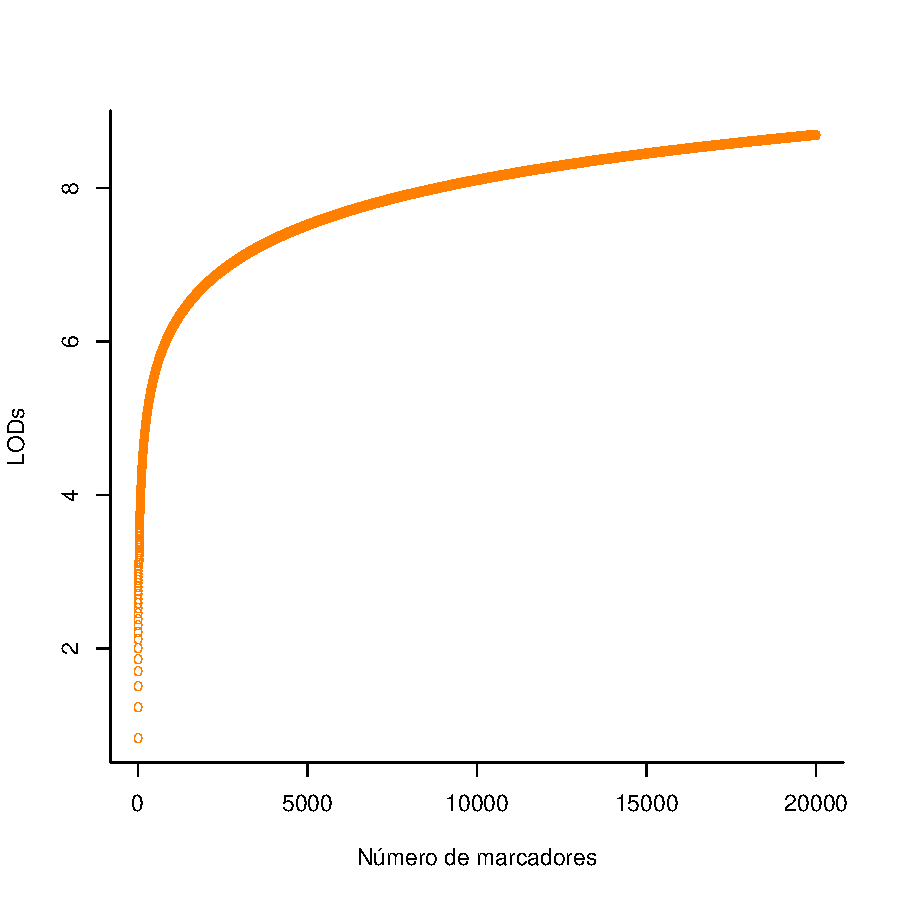
\includegraphics[scale=0.35]{figuras/graphical_model.pdf}
  \caption{In in tellus lacus. Sed aliquet efficitur efficitur.
    Maecenas posuere nulla eros. Pellentesque habitant morbi tristique
    senectus et netus et malesuada fames ac turpis egestas.
    Suspendisse ullamcorper diam eu tortor volutpat pharetra. Mauris
    eget purus non tortor convallis hendrerit. Suspendisse lacinia
    tincidunt nulla ut pretium. Aliquam nisi lorem, auctor vel nibh a,
    pharetra egestas est.}
  \label{fig:1}
\end{figure}

Nunc sed urna non augue placerat molestie. Donec ornare convallis
ultricies. Etiam ornare, nisi vitae vehicula posuere, odio nibh
tincidunt augue, ac scelerisque odio urna vel magna. Maecenas
consequat risus eu egestas mollis. Fusce tempus metus eu sapien
blandit, quis bibendum purus semper. Sed faucibus augue a nibh semper,
vel condimentum quam placerat. Morbi pulvinar interdum nibh, eu mattis
lorem iaculis et. Suspendisse iaculis quis ex in sodales. 

Donec ut gravida ipsum. Nunc ante ligula, accumsan eget lorem eget,
tincidunt semper felis. Nullam id enim non augue facilisis viverra.
Proin eu enim sed tortor iaculis pulvinar vitae nec risus. Phasellus
dolor tortor, faucibus vitae vulputate eget, malesuada ac neque. Nulla
ac tincidunt dui. Aliquam sed ligula consectetur, maximus eros et,
euismod sapien. Sed id auctor nisl. Vivamus et congue ligula. Aenean
ut blandit tortor. In interdum, urna ut blandit imperdiet, odio turpis
suscipit nulla, in porttitor est leo ac neque. Lorem ipsum dolor sit
amet, consectetur adipiscing elit. 

Integer sit amet turpis volutpat, laoreet massa non, rutrum justo.
Pellentesque egestas arcu sit amet viverra facilisis. Ut faucibus
vitae risus eget tristique. Morbi semper viverra laoreet. Curabitur
pharetra massa sed dolor suscipit, eget cursus nisl vestibulum.
Suspendisse potenti. Nullam sit amet maximus mi. Nullam non mauris
quis mi tincidunt eleifend. Nulla non nulla ac urna scelerisque
consectetur. Nullam bibendum dui in tellus tincidunt, nec posuere nisl
fermentum. Nam ut orci sed libero mattis fringilla ut sed ex. Nunc leo
lorem, vulputate malesuada fermentum sed, porta a odio. Vivamus vitae
massa luctus, posuere ante sed, consequat nunc. 

Phasellus tincidunt tincidunt magna, vitae aliquam arcu accumsan vel.
Nulla condimentum nibh et tortor gravida maximus. Donec nec tempor
sem, eu porttitor neque. Vivamus ultricies lacinia consectetur. Nulla
fringilla risus a dolor feugiat elementum. Morbi lectus nunc, lacinia
et ante quis, tempus tincidunt nulla. Nullam ac scelerisque eros, vel
faucibus sem. Praesent ac volutpat urna. Etiam nisl libero, elementum
quis risus non, placerat scelerisque leo. Donec eleifend in elit eget
auctor. Aenean nec pretium odio, id blandit dui. Nulla facilisi. 

Phasellus posuere mi felis, ac mattis tortor pretium non. Morbi
aliquam egestas enim vitae sagittis. Quisque id ligula tincidunt,
gravida eros a, tristique lectus. Proin eget dolor mollis, aliquet
turpis vel, rutrum tortor. Duis nec molestie mauris. Nulla facilisis
gravida nulla eget pulvinar. Maecenas lorem eros, porttitor vel arcu
id, sollicitudin volutpat felis. 

Vestibulum mauris justo, viverra ut massa ut, lacinia euismod eros.
Nulla semper tempor fringilla. Donec pharetra, mauris ac mollis
posuere, magna ipsum porta orci, quis maximus lectus lacus at eros.
Vestibulum posuere, ipsum nec lobortis sagittis, nibh quam pretium ex,
id bibendum neque massa sed ex. Integer nec magna elit. Donec diam
velit, rutrum nec orci vitae, fermentum feugiat lacus. Curabitur
tincidunt, turpis nec ornare imperdiet, lacus velit euismod purus, et
viverra felis erat vel augue. Aenean imperdiet eros eget orci egestas
rutrum in non augue. Duis quam lacus, fringilla a enim non, cursus
pretium elit. Integer in enim ac ligula imperdiet egestas. Morbi vel
tincidunt tellus, quis pretium elit. Ut vel egestas leo, sed luctus
urna. Etiam condimentum vitae purus non varius. In nulla nibh,
convallis sed dignissim non, convallis non purus. Cras non nisl nec
massa gravida congue. 

Sed sed luctus arcu, sit amet porta libero. Duis volutpat mauris
risus, eu rutrum lorem posuere in. Phasellus sit amet magna sodales,
commodo diam quis, mollis elit. Interdum et malesuada fames ac ante
ipsum primis in faucibus. Ut tempor consequat sem. Sed congue sapien
sit amet urna consequat, lacinia rutrum quam eleifend. Donec vel
sapien id sem malesuada consectetur quis ut neque. Vestibulum lacinia
ullamcorper ornare. 

Duis ac sollicitudin magna, non maximus lectus. Curabitur faucibus
lorem in ex cursus, a hendrerit est maximus. Vestibulum aliquet lectus
quis arcu volutpat, id sollicitudin nisi ullamcorper. Sed interdum
orci sed lacus dignissim, sed facilisis nibh facilisis. Duis aliquet
dolor sed nunc tincidunt, vitae imperdiet mauris ultricies. Fusce eget
quam nec enim molestie pulvinar. Sed convallis vulputate nibh, cursus
malesuada dui consectetur vel. In lorem dolor, blandit vitae dictum
fringilla, auctor sit amet nisl. Integer laoreet tellus ac felis
ultricies, vitae imperdiet odio volutpat. Nulla ac tortor bibendum,
imperdiet libero vel, tincidunt massa. Proin lobortis semper semper.
Pellentesque sollicitudin lobortis magna, ac dapibus risus ullamcorper
quis. Mauris cursus urna velit, eget tincidunt massa egestas sit amet. 

Fusce egestas, elit in mattis tempor, nisi felis rutrum sapien, et
pretium nunc diam sit amet nibh. Donec libero purus, consectetur ut
dapibus in, condimentum in arcu. Mauris venenatis felis mi, eget
elementum ligula porta facilisis. Proin elit libero, varius sit amet
orci id, ultrices sollicitudin felis. Suspendisse vulputate dui id sem
eleifend, sed hendrerit tortor cursus. Maecenas suscipit libero ut
accumsan volutpat. Etiam efficitur faucibus metus vel iaculis. Donec
vel sem sit amet odio tincidunt molestie consectetur et risus. Vivamus
eleifend massa vitae velit semper suscipit. Duis ut feugiat augue.
Cras et eros ultrices, eleifend turpis ut, pulvinar libero. Donec
lectus justo, malesuada fringilla bibendum vitae, convallis vel dolor.
Aliquam eu ex non mauris pretium viverra. Proin a nisl eget metus
commodo feugiat. Suspendisse sit amet risus gravida risus convallis
placerat.

\begin{figure}[htb]
  \centering
  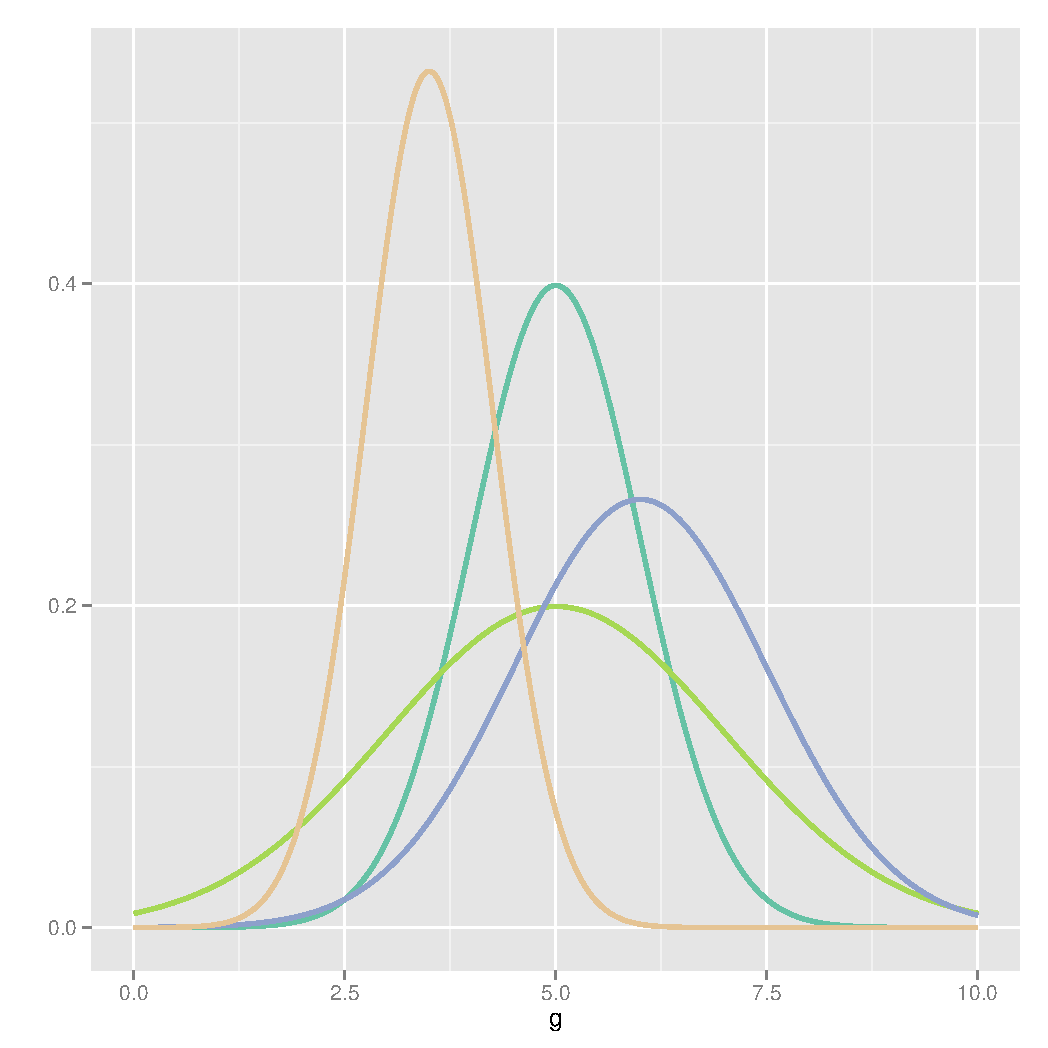
\includegraphics[scale=0.45]{figuras/distributions.pdf}
  \caption{Etiam ut bibendum sapien, id lacinia nisl. In hac
    habitasse platea dictumst. In congue diam diam. Proin quis risus
    tincidunt, placerat eros vel, tristique metus. Quisque mi mi,
    hendrerit vel arcu at, pharetra ultrices tortor. Phasellus
    euismod, nisl dictum malesuada aliquet, tortor elit commodo magna,
    at fermentum enim dolor ut purus. Nam bibendum sapien ut justo
    ullamcorper hendrerit.}
  \label{fig:2}
\end{figure}


\begin{table}
\centering
\caption{Cras eget congue velit, euismod cursus tortor. Donec
  facilisis dolor in ex suscipit commodo. Donec at vulputate est.
  Mauris placerat lorem ipsum, vel scelerisque mi aliquam sit amet.
  Nulla at elit rutrum sem gravida sodales. Maecenas vitae pulvinar
  nunc.}
\begin{tabular}{clr} 
\hline
Um & Dois & Três\\
\hline
1 & 2 & 3 \\
One & Two & Three\\
\hline
\label{Tab:result}
\end{tabular}
\end{table}




\chapter{Discussão}

In this work we used Phasellus vitae dui eget leo tristique accumsan
nec quis purus. In ac dapibus risus. Curabitur feugiat massa in
aliquet tincidunt. Morbi congue quis lorem vitae finibus. Vestibulum
euismod nunc et est bibendum rutrum. Maecenas lorem enim, porttitor eu
justo eget, lacinia rutrum massa. Quisque id commodo arcu. 

Nulla finibus magna eu eros tincidunt facilisis. Fusce aliquam ligula
quis dolor faucibus dictum. Phasellus dictum erat ipsum, ac euismod
quam auctor vel. Ut sit amet tempus mi. Morbi vitae lectus vel leo
ornare imperdiet vitae non sem. Nullam posuere eros nisl, ut venenatis
leo vehicula vel. Sed imperdiet eget erat ac porta. Morbi feugiat
semper justo, mollis hendrerit justo convallis eget. Suspendisse
condimentum eros augue, at rhoncus lectus laoreet id. Fusce mattis
aliquet magna sed porttitor. Mauris id enim neque. Pellentesque
habitant morbi tristique senectus et netus et malesuada fames ac
turpis egestas. Nam convallis cursus risus, sit amet tincidunt lacus
pretium molestie. Proin cursus sem faucibus risus viverra euismod. Cum
sociis natoque penatibus et magnis dis parturient montes, nascetur
ridiculus mus. Mauris non auctor mauris, vitae ultrices sem. 

Pellentesque habitant morbi tristique senectus et netus et malesuada
fames ac turpis egestas. Suspendisse euismod, dolor a lacinia tempor,
sem ipsum aliquet nulla, vitae egestas dui ligula in purus. In nisl
dui, venenatis ornare lorem sit amet, fringilla eleifend elit.
Pellentesque rutrum eros eget massa accumsan, id mollis sapien
dapibus. Pellentesque fermentum commodo lectus. Proin risus dui,
ultricies ac pulvinar at, mollis eget leo. Curabitur consequat elit eu
quam pretium volutpat a eget metus. Integer ac lacus non nibh congue
dictum vel nec orci. Ut ante felis, tristique eget accumsan a,
vulputate vitae ipsum. Pellentesque lobortis, leo elementum faucibus
scelerisque, turpis dolor efficitur tortor, quis scelerisque sem
lectus vitae tortor. Sed finibus sollicitudin blandit. Morbi vitae
efficitur nulla, non ultrices nulla. Nunc aliquet lectus in dignissim
mattis. 

Nullam eget lacinia libero. Phasellus faucibus bibendum nulla ac
fringilla. Nulla in nisl vitae purus laoreet feugiat. In imperdiet leo
ac consectetur tempor. Aenean hendrerit nunc at metus venenatis, sit
amet aliquet erat pulvinar. Mauris eu efficitur ex. Ut egestas
tristique tortor, eu hendrerit leo feugiat ultrices. Aenean euismod
facilisis consequat. Phasellus lobortis massa quis ipsum tincidunt
sodales. Aenean luctus nec velit vitae fermentum. 

Nunc dictum iaculis rutrum. Ut tincidunt libero est, in volutpat diam
posuere rutrum. Sed eu faucibus nisi. Duis id semper nisi. Maecenas
mollis, libero id vestibulum mattis, mauris nibh sollicitudin arcu, eu
cursus neque elit eget quam. Aliquam id accumsan massa. Duis placerat,
justo eu ultrices vehicula, nisi orci ullamcorper metus, sed egestas
erat erat quis justo. Proin eget porta turpis. Maecenas semper nisi ac
augue laoreet commodo. Phasellus eros eros, placerat vel dictum ut,
porta pharetra nunc. Morbi ut lorem imperdiet, mollis nisl et,
consequat lacus. Vivamus eros orci, dictum eget felis eget, maximus
ullamcorper quam. Maecenas porta placerat nisi id hendrerit. Nunc in
maximus lorem, ac suscipit velit. 

Integer convallis, metus vulputate blandit faucibus, est lacus
eleifend dolor, in aliquet arcu diam vel tortor. Sed ullamcorper
bibendum turpis eu gravida. Aenean ac tellus in massa bibendum
condimentum nec et libero. Vivamus ut elit consectetur, maximus tellus
eu, lacinia magna. Fusce venenatis diam nec sem egestas, non semper
felis semper. Aliquam cursus lectus dictum elementum sodales. Maecenas
aliquet magna ut finibus facilisis. Sed aliquet ante erat, nec aliquam
purus sagittis ac. Suspendisse hendrerit viverra enim, id sollicitudin
ex vestibulum non. Cras vitae ligula odio. Vestibulum porttitor mauris
eget elementum consectetur. Nullam in mi commodo, rhoncus metus vel,
vehicula diam. 

Sed interdum scelerisque orci a vehicula. Etiam ultrices nulla nec est
dictum hendrerit vitae id lacus. Proin condimentum nisl vel nunc
consectetur fermentum et id ligula. Ut id diam euismod metus tristique
interdum id non erat. Proin ut eros ligula. Donec est tellus, pulvinar
eu maximus ac, bibendum sit amet augue. Pellentesque egestas odio vel
augue cursus, vel ullamcorper est tempor. Nulla porta imperdiet ligula
non blandit. Fusce viverra neque ac enim viverra, id finibus nisl
vehicula. Maecenas ligula nunc, fringilla non orci eu, aliquam
malesuada dolor. Ut in purus nec felis aliquam faucibus eu sed lorem.
Maecenas sed mauris eget erat venenatis gravida in sit amet augue.
Curabitur condimentum efficitur nisi eget ultrices. Nam quis tortor
ante. In eget nulla et tortor tincidunt tempor. Nullam posuere
accumsan sapien at tincidunt. 

Curabitur nec imperdiet odio, sit amet varius eros. Mauris vulputate,
erat ut porta vulputate, metus risus sagittis mauris, sed semper orci
lectus in elit. Nulla rutrum ultricies quam, et consectetur nunc
commodo sed. Vestibulum iaculis sollicitudin scelerisque. In id
efficitur ligula. Sed et mi eleifend, dignissim quam et, condimentum
ante. Vestibulum ante ipsum primis in faucibus orci luctus et ultrices
posuere cubilia Curae; Mauris volutpat augue eu ipsum vestibulum, et
porta dolor gravida. Donec id sapien in metus lacinia ultrices sit
amet at ante. Mauris vestibulum nunc sit amet enim volutpat luctus.
Vivamus tincidunt ex at lacus laoreet lacinia. 

Proin ipsum lorem, accumsan quis gravida a, feugiat id dolor. Aenean
nec pellentesque velit. Vivamus vitae mollis metus, vitae laoreet
felis. Maecenas vitae purus et orci lacinia feugiat sed eget lectus.
Sed finibus at est sit amet porttitor. Morbi vitae posuere velit.
Nulla sed rhoncus nulla. Cras suscipit sit amet tellus non sagittis.
Phasellus mi sem, mollis eget fringilla ut, accumsan sed enim. 

Integer nibh lacus, sollicitudin at sodales in, elementum eu metus.
Quisque vitae quam at nulla faucibus volutpat. Pellentesque venenatis
lobortis convallis. Maecenas porttitor ex sit amet nibh fermentum
ultrices. Cum sociis natoque penatibus et magnis dis parturient
montes, nascetur ridiculus mus. Vestibulum gravida euismod erat. Nam
sed est laoreet, elementum nibh a, blandit ligula. Vestibulum
tincidunt eget nisl ornare ornare. Donec et augue vitae sapien
convallis placerat sit amet ut velit. Cras feugiat, mauris sed pretium
venenatis, elit lectus fermentum nulla, nec rhoncus nulla mi a urna.
Proin interdum massa eget risus pharetra, et molestie ligula molestie.
Donec egestas dolor id condimentum maximus. Aliquam in felis vehicula,
finibus lacus eget, ornare sapien. In iaculis elit turpis, ut blandit
lectus blandit suscipit. Mauris ac commodo quam. 

Ut semper eu mi et consectetur. Duis malesuada ex id mi posuere, ac
hendrerit massa cursus. Aliquam congue tortor ac turpis facilisis
viverra. Nam id lacinia justo, sed consectetur metus. Praesent nec
molestie lorem. Nulla enim erat, molestie vitae enim sed, finibus
eleifend odio. Cras aliquet arcu at aliquam fringilla. Nulla interdum
ultricies odio at mattis. Nam sapien justo, auctor eget fringilla at,
interdum at nibh. Proin lobortis pellentesque feugiat. Ut fermentum
orci at eros aliquet varius. Cras feugiat eget justo vitae tempus.
Quisque tellus urna, molestie at tempor in, dapibus sed tellus. Mauris
id purus tellus. Nulla tincidunt metus vitae dictum congue. 

Nullam venenatis leo non mauris viverra rutrum. Pellentesque at turpis
at purus tincidunt consectetur. Sed sed neque arcu. Quisque tempus
justo quis finibus condimentum. Ut tincidunt urna eu purus fringilla,
a aliquam mauris auctor. Vivamus ultrices luctus nulla vel tempor.
Vivamus consectetur facilisis nulla a bibendum. Duis dapibus auctor
tempus. Sed eget ullamcorper nulla. Aliquam scelerisque velit nec
consectetur tempor. Nullam elit arcu, pellentesque nec convallis eu,
sodales eget magna. Nulla lobortis congue magna eget vulputate. Duis
ut pellentesque ante. 

Aliquam volutpat eros augue, vel tempor sapien auctor et. Suspendisse
fringilla fermentum massa eget tincidunt. Aliquam ante enim, hendrerit
ut enim ac, tincidunt iaculis ex. Donec leo est, vehicula a tincidunt
tempor, porta at velit. Etiam euismod porttitor metus vel gravida.
Donec rutrum aliquam tincidunt. Nulla commodo ut lectus nec porttitor.
Curabitur tincidunt magna sollicitudin, facilisis tortor ac, blandit
massa. Quisque eu imperdiet lacus, sit amet iaculis eros. Etiam mi
elit, dictum vitae ornare et, lacinia vitae mi. Curabitur dignissim
tortor finibus lectus fringilla hendrerit.



% Referências. 
% O template faz uso do BibTex. Verifique o formato
% apropriado para o seu caso. Abaixo, é apresentado um exemplo para o
% formato de citação da revista Genetics. O estilo correspondente está
% localizado no arquivo genetics.bst (fornecido pela revista), que
% está no diretório "referencias". Use o .bst adequado para seu
% trabalho, mudando o estilo abaixo, como indicado. Já a base de dados
% de referências, no formato BibTeX, está no arquivo bibliografia.bib
% (também no diretório "referencias"). Use os arquivos apropriados
% para o seu caso.

\renewcommand\bibname{Referências} %Muda "Referência Bibliográficas" para Referências
\bibliographystyle{./referencias/genetics} %Localização do arquivo genetics.bst
\bibliography{./referencias/bibliografia} %Localização do arquivo bibliografia.bib
\clearpage

%%%%%%%%%%%%%%%%%%%%
% Parte Pós-textual
% Apêndices e Anexos

% Apêndices (opcionais). Edite da forma desejada.
% Não mude esta parte
\chapter*{Apêndices}
\addcontentsline{toc}{chapter}{Apêndices}
\counterwithout{figure}{chapter}
\counterwithout{table}{chapter}
\renewcommand{\thefigure}{A.\arabic{figure}}
\renewcommand{\thetable}{A.\arabic{table}}


% Insira aqui seus Apêndices

\section*{Apêndice I}

Nulla condimentum vulputate porttitor. Nulla sollicitudin ante vel
orci fringilla suscipit. Sed dolor diam, vulputate eu iaculis non,
lobortis vel neque. Vivamus sit amet lectus mauris. Sed odio libero,
finibus sed iaculis nec, fermentum a mauris. Vivamus ac arcu mauris.
Donec molestie accumsan pulvinar. Sed feugiat in tortor vel porta.
Donec sed sem posuere, suscipit nunc a, posuere diam.

\begin{table}[h]
\centering
\caption{Fusce lacinia pretium maximus. Vestibulum sagittis tempor
  ligula, vitae ultricies ipsum congue sit amet. Phasellus convallis
  elit quis magna molestie placerat. Morbi id volutpat arcu. Sed
  laoreet tortor eget turpis pulvinar rhoncus. Praesent eget leo ut
  velit tristique tristique et vel mi.}
\begin{tabular}{clr} 
\hline
Quatro & Cinco & Seis\\
\hline
4 & 5 & 6 \\
Four & Five & Six\\
\hline
\label{Tab:A1}
\end{tabular}
\end{table}


\begin{figure}[htb]
  \centering
  
\includegraphics[scale=0.10]{figuras/spiderman.jpg}
  \caption{Aliquam vel tortor vitae metus posuere gravida. Maecenas
    ultricies enim mauris, ut ultrices justo pretium sed. Praesent
    bibendum, lorem sit amet auctor fringilla.}
  \label{fig:A1}
\end{figure}


\section*{Apêndice II}

Vivamus sit amet lectus mauris. Sed odio libero, finibus sed iaculis
nec.


% Anexos (opcionais). Edite da forma desejada.
% Não mude nada aqui
\chapter*{Anexos}
\addcontentsline{toc}{chapter}{Anexos}
\counterwithout{figure}{chapter}
\counterwithout{table}{chapter}
\renewcommand{\thefigure}{anexo\arabic{figure}}
\renewcommand{\thetable}{anexo\arabic{table}}


% Insira aqui seus Anexos

\section*{Anexo A}

Vestibulum blandit vestibulum porta. Proin scelerisque eros molestie
accumsan ultrices. Sed augue felis, hendrerit ac nibh vitae, aliquet
vehicula massa. Etiam in scelerisque dolor, et interdum mauris. Nulla
facilisis ac ligula a pharetra.

\section*{Anexo B}

Etiam in scelerisque dolor, et interdum mauris.


\end{document}
